\subsection{Loi normale - Rectangles et coins}
Pour un très grand nombre de tirages aléatoires, la méthode Rectangle et coins ou \linebreak Rectangle-wedge-tail est encore plus rapide que la méthode polaire.

Pour cette méthode on n'utilise que la partie droite de la distribution:
\[f(x)=\sqrt{\frac{2}{\pi}}e^{-\frac{x^2}{2}}\]

Nous allons également considérer la distribution comme une somme pondérée de fonctions:
\[f(x)=p_1f_1(x)+p_2f_2(x)+...+p_nf_n(x) \qquad \sum\limits_{i=1}^{n} p_i=1\]

Certaines densités de fonction $f_j(x)$ peuvent être plus compliquées à calculer, on pourra donc leur attribuer un $p_j$ plus petit afin de rendre l'algorithme plus efficace.
A présent, divisons l'aire sous notre demi-courbe en, par exemple, 31 parts.

\begin{center}
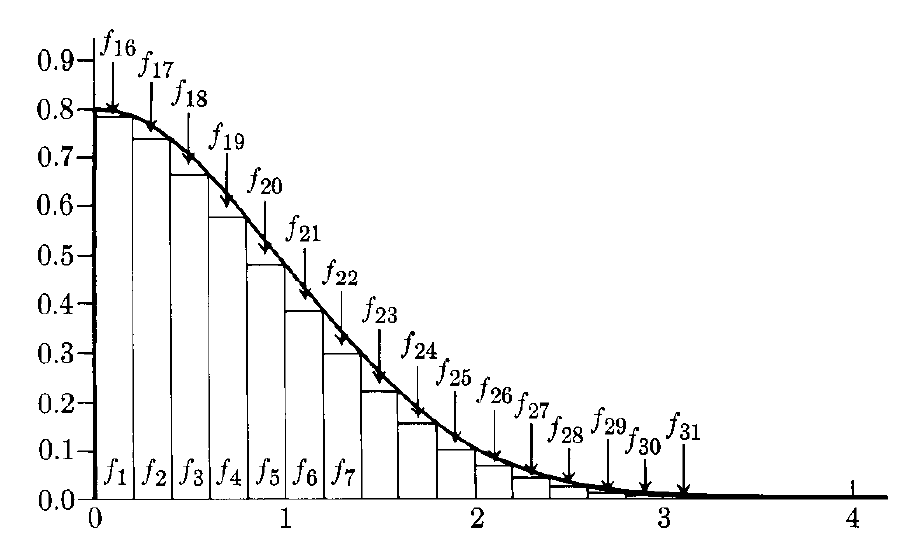
\includegraphics[width=10cm]{normal}
\end{center}

On remarque
\begin{itemize}
\item 15 rectangles représentant $p_1f_1(x),...,p_{15}f_{15}(x)$
\item 15 coins (au dessus des rectangles) représentant $p_{16}f_{16}(x),...,p_{30}f_{30}(x)$
\item 1 queue de la distribution représentant $p_{31}f_{31}(x)$
\end{itemize}

Les parties rectangulaires sont des distributions uniformes. Par exemple, $f_3(x)$ représente une variable aléatoire uniformément distribuée entre $\frac{2}{5}$ et $\frac{3}{5}$ (voir figure). L'aire du j-ième rectangle est
\[p_j=\frac{1}{5}f(\frac{j}{5})=\sqrt{\frac{2}{25\pi}}e^{-\frac{j^2}{50}} \qquad 1\leq j\leq 15\]
Dans ce cas on peut générer $U$ suivant une loi uniforme dans [0,1[ et prendre \[X=\frac{1}{5}U+S\qquad \text{où }S=\frac{j-1}{5}\text{ avec une probabilité }p_j\]

Notons que $p_1+p_2+...+p_{15}=0.9183$ et donc que cette zone représente près de 92\% de la génération. Pour les 8\% restant il faut générer une des distributions de \og coins\fg{}, $f_{16},...,f_{30}$.

On remarque que lorsque $x<1$ $(f_{16},...,f_{20})$, la concavité de la courbe est vers le bas tandis que si $x>1$ $(f_{21},...,f_{30})$, la concavité de la courbe est vers le haut.
Cependant la courbe est raisonnable et on peut l'encadrer entre deux droites parallèles comme montré ci-dessous.

\begin{center}
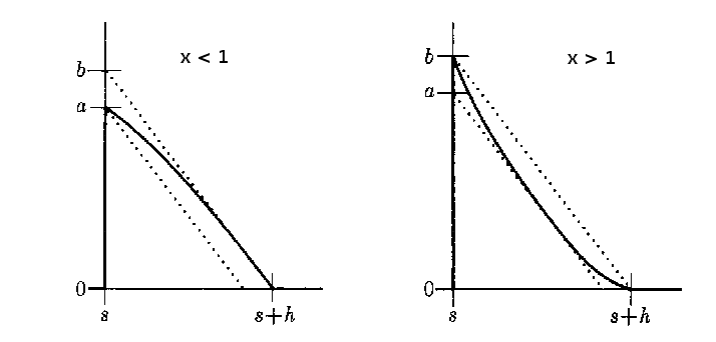
\includegraphics[width=12cm]{coins}
\end{center}

\begin{itemize}
	\item Pour $x<1$, on prend la tangente au point de droite et sa parallèle qui passe par l'autre point.
	\item Pour $x>1$, on joint les deux points extrêmes et on prend la tangente parallèle.
\end{itemize}

On obtient alors
\[
		\begin{aligned}
		a-\frac{b(x-s)}{h}&\leq& f(x) &\leq& b-\frac{b(x-s)}{h}\\
		\frac{a}{b} &\leq& \frac{1}{b}f(x)+\frac{(x-s)}{h} &\leq& 1
		\end{aligned}
\]

\begin{enumerate}
	\item On génère $U$ et $V$ uniformément dans [0, 1[ avec $V>U$ (sinon on échange)
	\item Si $V\leq \frac{a}{b}$, on va à l'étape 4.
	\item Si $V\leq U+(\frac{1}{b})f(s+hU)$, on retourne à l'étape 1. (si $\frac{a}{b}$ est proche de 1, on passera rarement dans ce cas)
	\item $X=s+hU$
\end{enumerate}

Vérification: voir cours, slide 90

Il ne nous reste plus qu'à traiter le cas de la queue de la distribution $f_{31}$. Ce cas ne se réalise qu'environ une fois sur 370.

\begin{itemize}
	\item Soit $f(x)$ une densité de probabilité suivant laquelle on génère des nombres aléatoires.
	\item Soit $g(x)$ une densité de probabilité suivant laquelle il est facile de générer des nombres aléatoires.
	\item Soit $f(x)\leq c\ g(x)$ où c est le plus petit possible $(c\geq 1)$
\end{itemize}

Algorithme pour générer des nombres selon $f(x)$:
\begin{enumerate}
	\item On génère $X$ selon $g(x)$.
	\item On génère $U$ uniforme dans [0,1[.
	\item Si $\frac{f(X)}{c\ g(X)}\leq U$ alors on retourne en 1 sinon on accepte X.
\end{enumerate}

La probabilité de rejeter X est alors
\[q=\int_{-\infty}^{+\infty} (g(t)dt\ (1-\frac{f(t)}{cg(t)}))=1-\frac{1}{c}\]

La probabilité d'accepter X est $\frac{1}{c}$

La probabilité d'accepter X généré suivant $g(x)$ (Point 3 de l'algo): $\frac{f(x)}{c*g(x)}$

La densité de probabilité de X: $f(x)=\frac{g(x)*\frac{f(x)}{c*g(x)}}{\frac{1}{c}}$

Prenons un exemple:\\
Soient
\[
f(t)=\frac{e^{-\frac{t^2}{2}}}{\int_3^{+\infty} e^{-\frac{u^2}{2}}du} \quad \text{et} \quad g(t)=a t e^{-\frac{t^2}{2}}
\]

On doit déterminer $a$ et $c$
\[
\int_3^{+\infty}g(t)dt=1=a\int_3^{+\infty}te^{-\frac{t^2}{2}}dt=\frac{a}{2}\int_9^{+\infty}e^{-\frac{t^2}{2}}dt^2=a\left [-e^{-\frac{x}{2}}\right ]_9^{+\infty}
\]

On tire donc que $a=e^{\frac{9}{2}}$, $g(t)=te^{\frac{9-t^2}{2}}$

La fonction de répartition de $g(x)$ notée $G(x)$:
\begin{align*}
G(x)=\int_3^xte^{\frac{9-t^2}{2}}dt &= \frac{1}{2}\int_9^{x^2}e^{\frac{9-t^2}{2}}dt^2\\
&= \frac{1}{2}e^{\frac{9}{2}}\int_9^{x^2}e^{-\frac{t^2}{2}}dt\\
&= e^{\frac{9}{2}}\left [-e^{-\frac{x^2}{2}}+e^{-\frac{9}{2}}\right ]\\
&= 1-e^{\frac{9-x^2}{2}}\\
&= y
\end{align*}

On peut alors générer $z=1-y=e^{\frac{9-x^2}{2}}$ dans $[0,1[$ et on trouve $x=\sqrt{9-2\ln{z}}$

Il nous manque encore $c$:
\begin{align*}
\frac{f(t)}{cg(t)} &=\frac{e^{-\frac{t^2}{2}}}{c\left [ \int_3^{+\infty} e^{-\frac{u^2}{2}}du\right ]te^{\frac{9-t^2}{2}}} \\
&=\frac{e^{-\frac{9}{2}}}{ct\int_3^{+\infty}e^{-\frac{u^2}{2}}du} \leq 1\\
&\Rightarrow c \geq \frac{e^{-\frac{9}{2}}}{t\int_3^{+\infty}e^{-\frac{u^2}{2}}du}
\end{align*}

On peut prendre $c=\frac{e^{-\frac{9}{2}}}{3\int_3^{+\infty}e^{-\frac{u^2}{2}}du}$

On accepte alors X si $U<\frac{F(X)}{cg(X)}=\frac{3}{X}$
\vspace{0.3cm}

\begin{figure}[h]
	\centering
  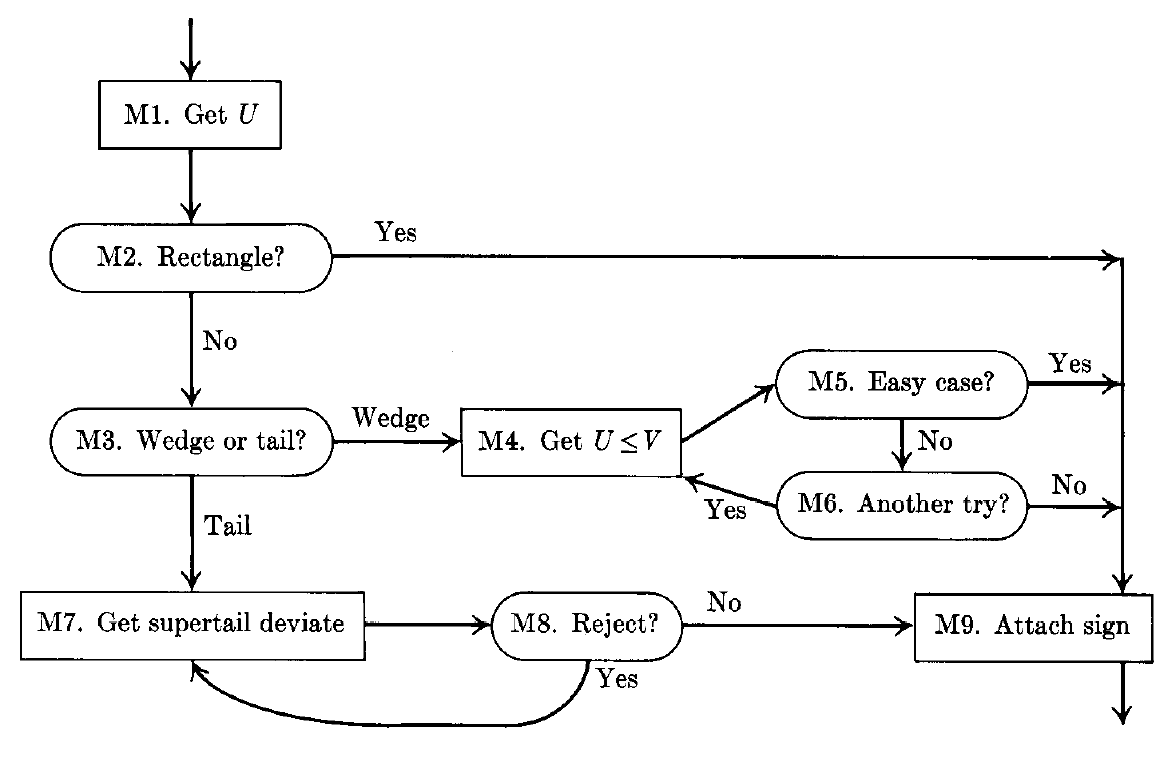
\includegraphics[width=12cm]{graphe}
	\caption{L'algorithme en résumé}
\end{figure}